\author{Autor: Patrick Künzel}
\chapter{\ac{RSA}}
\section{Motivation}
Online-Zahlungen sind aus unserem Alltag nichtmehr wegzudenken. Aus Paypals
letztem Quartalsbericht für das Jahr 2015 konnte man entnehmen, dass allein am
"`Cyber Monday"' 450 Zahlungen pro Sekunde verarbeitet wurden. Das sind circa
1,6 Millionen Geldbewegungen in einer Stunde.\footnote{Vgl. \citet{MotleyFool}}
Für Hacker demnach ein Paradies, um Nutzerdaten oder Geldflüsse zu beeinflussen.
Um dieses Szenario zu vermeiden, werden z.B. Online-Transaktionen durch
verschiedene Verschlüsselungsverfahren (auch Kryptosysteme genannt) gesichert.
Eines dieser Kryptosysteme ist das "`RSA-Verfahren"'. Es ist eines der
ältesten Verfahren und in der Kategorie der \emph{asymmetrischen
Verschlüsselungsverfahren} einzuordnen. RSA kommt z.B.
bei E-Mail-Verschlüsselungen (OpenPGP, S/MIME) oder der Telefonie zum Einsatz.
Dieses Kapitel beschäftigt sich mit dem Konzept/ der Funktionsweise von RSA,
seiner mathematischen Durchführung/Besonderheiten (anhand eines Beispiels
dargestellt) und der Sicherheit.
\section{Einleitung}
Das RSA-Verfahren wurde von Ron \textbf{R}ivest, Adi \textbf{S}hamir und Leonard \textbf{A}dlemann 
entwickelt. 1977 entstand die erste öffentliche Version des
Verschlüsselungsverfahrens.\footnote{Vgl.
\citet{RSAWiki}} Es ist verwandt mit dem "`Rabin-Kryptosystem"'. RSA basiert auf
2 wichtigen Grundideen:
\begin{enumerate}
  \item Public-Key Verschlüsselung: \newline
  Der Kerngedanke besteht, anders als bei den symmetrischen
  Verschlüsselungsverfahren, daraus, 2 verschiedene Schlüssel für eine
  Verschlüsselung zu verwenden. Die Schlüssel zum
  Verschlüssen sind öffentlich, während der
  Schlüssel zum Entschlüsseln privat ist und nicht weitergegeben werden darf.
  Das Public-Key-Verfahren besteht formal aus drei verschiedenen Algorithmen:
  \begin{itemize}
    \item Dem Schlüsselerzeugungsalgorithmus, welcher die Grundlage für die
    Verschlüsselung schafft und den öffentlichen und privaten Schlüssel
    generiert.
    \item Dem Verschlüsselungsalgorithmus, der mithilfe des öffentlichen
    Schlüssels den Klartext in einen Geheimtext umwandelt. Ein Klartext kann
    hierbei in mehrere Geheimtexte resultieren, je nachdem welchen öffentlichen
    Schlüssel man benutzt. $1:n$
    \item Dem Entschlüsselungsverfahren, welcher aus dem Geheimtext mittels
    des privaten Schlüssels den Klartext berechnet. Hier ist nur $1:1$ Zuordnung
    möglich, das bedeutet, dass ein Geheimtext nur mit einem bestimmten privaten
    Schlüssel entschlüsselt werden kann.
  \end{itemize}
  \item Digitale Signatur: \newline
	Das RSA-Verfahren kann ebenso zur Signierung von Nachrichten benutzt werden.
	Hierbei wird die Klartext-Nachricht des Senders mit dem Private-Key
	verschlüsselt und mit dem öffentlichen Schlüssel des Empfängers entschlüsselt. 
	Mit dem privaten Schlüssel eine Nachricht zu "`verschlüsseln"' ist keinerlei
	ein Widerspruch unter der Prämisse, dass $T = V$ (Klartext gleich Geheimtext)
	ist.
	\begin{displaymath}
	E(T) = C \ \ \ \ \ \footnote{Vgl. \citet{RSAAlgorithm} - S.
  1}
	\end{displaymath}
	\begin{center}
	\emph{E = Verschlüsseln (Encrypt); T = Text; C = Ciphertext (Geheimtext) }
	\end{center}
	Die Zahlen, welche die Nachricht repräsentieren unterscheiden keinen Klartext
	von einem Geheimtext. Die Interpretation des Lesers wiederum entscheidet, ob 
	der Text einen logischen Zusammenhang ergibt (dann ist es der sogenannte
	"`Klartext"') oder nicht (dann ist es der Geheimtext). Durch die
	Verschl+sselung mit dem privaten Schlüssel wird nun erreicht, dass wenn der
	Empfänger empfangenen Text entschlüsselt, er eine lesbare Nachricht zu Augen
	bekommt.
	\begin{displaymath}
	D(C) = D(E(T)) = T \ \ \ \ \ \footnote{Vgl. \citet{RSAAlgorithm} - S.
  2}
	\end{displaymath}
	\begin{center}
	\emph{E = Verschlüsseln (Encrypt); D = Entschlüsseln (Decrypt); T = Text; C =
	Ciphertext (Geheimtext) }
	\end{center}
	Schickt der Sender gleichzeitig die selbe Nachricht unverschlüsselt zum
	Empfänger, hat der Empfänger die Möglichkeit beide Nachrichten miteinander zu
	vergleichen.
	Sollten diese übereinstimmen, kann der Empfänger sicher sein, dass diese
	Nachricht von dem Inhaber des privaten Schlüssels gesendet worden ist. Die
	Integrität und Authentizität wird somit garantiert.
\end{enumerate}

Das Geheimrezept für eine starke Verschlüsselung bildet ein schwieriges
mathematisches Problem. Das bedeutet, dass man den Hinweg (Zahlen werden zu
einem Ergebnis verarbeitet) einer Berechnung einfach durchführen kann, aber der
Rückweg (vom Ergebnis zu den verwendeten Zahlen) sich als komplexes Problem
darstellt (Stichwort: \emph{Einwegfunktionen}). Ein
solches komplexes Problem wäre die Primfaktorzerlegung, auf dessen das
RSA-Verfahren beruht. Bei der Primfaktorzerlegung werden 2 verschiedene
Primzahlen miteinander multipliziert, dies ist der einfache Teil. Aus dem
Produkt beide Primzahlen zu ermitteln, gestaltet sich jedoch als
weitaus schwieriger. Es gilt: "`Je größer der Multiplikator und der
Multiplikand, desto schwieriger die Ermittlung der einzelnen Bestandteile aus
dem Produkt"'. In der Praxis werden Primzahlen mit mehreren 100 Dezimalstellen
verwendet.
\section{Funktionsweise}
Folgende Grafik veranschaulicht die Funktionsweise/den Ablauf des
RSA-Verfahrens. \newline
\begin{figure}[H]

\includegraphics[width=1\textwidth]{publickey.png}
\caption[Ablauf des RSA-Verfahren]{grafische Darstellung des RSA-Verfahren -
Quelle: http://pajhome.org.uk/crypt/rsa/intro.html, Stand 18.02.2016}
\end{figure}

Im Folgenden werden die einzelnen Schritt ausführlich erläutert.
  \subsection{Die Schlüsselgenerierung}
  Bevor Dateien ver- und wieder entschlüsselt werden können, wird zunächst der
  öffentliche und private Schlüssel kreiert. Dazu wählt man zwei
  unterschiedlich große Primzahlen \emph{p} und \emph{q} und bildet das Produkt
  \emph{n}, auch bekannt als \emph{RSA-Modul}.
  \begin{displaymath}
  N = p * q
  \end{displaymath}
  Danach wird $\phi(N)$ berechnet.
  \begin{displaymath}
  \phi(N) = \phi(p) * \phi(q) = (p-1) * (q-1)
  \end{displaymath}
  Als nächsten Schritt wählt man eine Zahl $e$ mit $1<e<\phi(N)$, wobei der
  größte gemeinsame Teiler von $e$ und $\phi(N)$ 1 sein muss. ($ggT(e,
  \phi(N)))=1$)
  Der öffentliche Schlüssel setzt sich nun aus den Werten $e$ und $N$ zusammen.
  \begin{displaymath}
  KeyOeffentlich = (e,N)
  \end{displaymath} 
  $p$, $q$ und $\phi(N)$
  dürfen nicht rausgegeben werden. \newline\newline
  Für den privaten Schlüssel bestimmt man $d$ mit 
  \begin{displaymath}
  e*d \equiv 1 \ mod(\phi(N))
  \end{displaymath}
  und löst die Gleichung $e*d+k*\phi(N)\equiv 1 \ mod(\phi(N))$ mit dem
  erweiterten euklidischen Algorithmus. Das x, welches man aus der Tabelle
  errechnet (für eine anschauliche Darstellung siehe nächsten Abschnitt) ist nun
  das Inverse-Element von $e$. Demnach haben wir nun alle benötigten Elemente
  für unseren privaten Schlüssel zusammen.
  \begin{displaymath}
  KeyPrivat = (d, N)
  \end{displaymath}
  \subsection{Verschlüsselung}
  Möchte man nun einen Klartext mit dem öffentlichen Schlüssel verschlüsseln, so
  gilt die Formel:
  \begin{displaymath}
  V = T^e \ mod(N)
  \end{displaymath}
  \subsection{Entschlüsselung}
  Um die Umkehrfunktion der Verschlüsselung zu bilden, ersetzen wir $e$ mit $d$
  aus dem privaten Schlüssel. Daraus ergibt sich:
  \begin{displaymath}
  T = V^d \ mod(N)
  \end{displaymath}
\section{Praktisches Beispiel}
\emph{Damit man das folgende Beispiel besser nachvollziehen kann, sei kurz
gesagt, dass Daten nicht nur durch Bitfolgen angesehen werden können, sondern
auch durch Zahlen. Für den Computer macht es keinen Unterschied, ob er das Zeichen "`C"'
als Bitfolge abspeichert oder den ASCII-Code von C - "`67"'. Für die
Verschlüsselung macht es jedoch einen großen Unterschied, da man mit Zahlen
mathematisch agieren kann, im Gegensatz zu Buchstaben. Nachteil dieser
Herangehensweise ist die Tatsache, dass sowohl Sender als auch Empfänger
das gleiche "`Dictionary"' benötigen, um aus der Zahlenbasis wieder einen reinen
Text zu gestalten. (zum Beispiel die
ASCII-Tabelle)}\newline\newline Nehmen wir an Alice möchte Bob eine
verschlüsselte Nachricht zukommen lassen.
Ihr Klartext $T$ enthält den Buchstaben "`C"'. C ist der dritte Buschstabe im
Alphabet, also wählen wir die 3. Somit ergibt sich $T = 3$.
Als nächstes werden die Schlüssel generiert. Hierzu denken wir uns zunächst 2
verschiedene Primzahlen aus und multiplizieren sie miteinander um das
Produkt $N$ herauszubekommen.
\begin{displaymath}
p = 5, q = 7 \rightarrow N = p * q = 35
\end{displaymath}
Danach bestimmen wir $\phi(N)$. Das besondere hierbei ist, dass $N$ aus
2 Primzahlen besteht. Für Primzahlen gilt: $ \phi(p) = p-1$. Somit gilt für
unser Beispiel:
\begin{displaymath}
\phi(N) = \phi(p) * \phi(q) = (p-1)*(q-1) = 4*6 = 24 
\end{displaymath}
Jetzt brauchen wir unser $e$. $e$ muss teilerfremd zu $\phi(N)$ sein. Wie im
Grundlagenteil erläutert, gilt für $e$ folgende Regel: 
\begin{displaymath}
e \in \mathbb{N} \ | \ ggT(e,N) = 1 \ \ \gets \  \ 1<e<\phi(N)
\end{displaymath}
Das $e$ stellt immer eine Primzahl dar, wobei nicht jede Primzahl teilerfremd
zu $e$ sein muss. In diesem Beispiel wäre 3 für $e$ keine gültige Primzahl da
$24/3 = 8$. In diesem Fall wird $e$ auf den Wert $e = 11$ gesetzt. Das
$e$ sollte zudem nicht allzu klein gewählt sein. Trotz einer erheblichen
Einbußung der Performance des Algorithmuses, ist es sehr unsicher, Zahlen wie 3
oder 17, zu verwenden. Falls ein Angreifer versuchen sollte sich das $\phi(N)$ durch
zurückrechnen herzuleiten, so wird es für ihn nicht leichter. Ebenso sollte es
vermieden werden $p$ oder $q$ als $e$ zu benutzen.
\newline\newline
Der öffentliche Schlüssel wäre somit $KeyOeffentlich = (11, 35)$.
\newline\newline
Im nächsten Schritt wird nun $d$ bestimmt. $d$ muss das Inverse von $e \
mod(\phi(N))$ darstellen, damit die allgemeine Formel $e*d \equiv 1 \
mod(\phi(N))$ gilt.
$e$ wurde so ausgesucht, dass es genau ein Inverses gibt. Um das Element zu berechnen
benötigen wir hier den erweiterten euklidischen Algorithmus. Dieser wurde im
Einleitungsteil umfassend erklärt. Als diophantische Gleichung ergibt sich:
\begin{displaymath}
11*x + 24 * y = 1
\end{displaymath}
Den Rechenweg der Gleichung erkennen Sie in Abbildung 2.\newline
\begin{figure}[H]
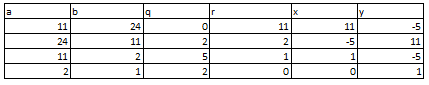
\includegraphics[width=1\textwidth]{eEA.png}
\caption[erweiterter euklidischer Algorithmus (Beispiel)]{eigene Darstellung
des erweiterten euklidischen Algorithmus zur diophantischen Gleichung $11*x +
24*y = 1$}
\end{figure}
Das x aus der Tabelle bildet das Inverse-Element, welches wir benötigen. An
dieser Stelle können 2 Besonderheiten auftreten.
\begin{enumerate}
  \item Wie in unserem Fall spiegelt unser $d$ auch unser $e$ wieder. Dies ist
  nicht einem Rechenfehler geschuldet, sondern der Tatsache der kleinen
  Schlüssellänge unseres Beispiels (6 Bit). Ab einer größeren Schlüssellänge
  unterscheiden sich $d$ und $e$ mit wachsender Wahrscheinlichkeit. Das es sich
  um keinen Rechenfehler handelt erkennt man später daran, dass die
  Zwischenergebnisse vor dem Modulo-Rechnen 2 unterschiedliche Zahlen sind.
  \item Es könnte ebenso der Fall auftreten, dass das x nach dem
  erweitereten euklidischen Algorithmus negativ ist. In diesem Fall darf man 
  den ermittelten Wert nocheinmal mod(N) rechnen, z.B. $-9 = 31 \ mod
  (40)$.\footnote{Vgl.
  http://www.onlinemathe.de/forum/RSA-Was-wenn-inverser-Schluessel-negativ-ist}
\end{enumerate}
Um zu überprüfen, ob man den erweiterten euklidischen Algorithmus richtig
verwendet hat, werden die Zahlen in die obige Gleichung eingesetzt.
\begin{displaymath}
11*11 + 24 * -5 = 121 - 120 = 1
\end{displaymath}
Unser privater Schlüssel laute demnach $KeyPrivat = (11,35)$.
\newline\newline
Nachdem wir nun unsere Schlüssel generiert haben, kann mit der Verschlüsselung
angefangen werden. Zur Verschlüsselung gilt die Formel $V = T^e \ mod(N)$, mit
der Bedingung das $T$ nicht größer als $N$ ist, sonst wäre das Modulo-Rechnen
beim Entschlüsseln nicht erfolgreich.
In diesem Beispiel laute die Verschlüsselungsformel wie folgt:
\begin{displaymath}
V = 3^{11} \ mod(35)
\end{displaymath}

Rechenweg:
\begin{displaymath}
3^{11} \ mod(35)
\equiv 3^3 *(3^2)^4 \ mod(35)
\equiv 27 * (9)^4 \ mod(35)
\equiv 27 * (11)^2 \ mod(35)
\equiv 27 * 121 \ mod(35)
\end{displaymath}
\begin{displaymath}
\equiv 27 * 16 \ mod(35)
\equiv 12
\end{displaymath}
\newline
Verschlüsselt ergibt der Klartext $T$ nun den Wert $V = 12$. Unser Buchstabe
"`C"' symbolisiert für einen Außenstehenden theoretisch nun den
Buchstaben "`L"'.
\newline\newline 
Um zu zeigen, dass der private Schlüssel trotz gleichem $d$ und $e$ stimmt,
können wir den Geheimtext wieder entschlüsseln.
Die Formel dazu lautet $T = V^d \ mod(N)$.

\begin{displaymath}
T = 12^{11} \ mod(35)
\end{displaymath}

Rechenweg:
\begin{displaymath}
12^{11} \ mod(35)
\equiv 12^1 * 12^2 * (12^2)^4 \ mod(35)
\equiv 12*144*144^4 \ mod(35)
\equiv 12*4*4^4 \ mod(35)
\end{displaymath}
\begin{displaymath}
\equiv 48*(4^2)^2 \ mod(35)
\equiv 13*(16)^2 \ mod(35)
\equiv 13*256 \ mod(35)
\equiv 13*11 \ mod(35)
\end{displaymath}
\begin{displaymath}
\equiv 143 \ mod(35)
\equiv 3
\end{displaymath}

Man erkennt, dass unser Klartext $T = 3$ lautet und somit gleich unserer
Ausgangszahl ist. Hiermit wurde bewiesen, dass die Schlüssel korrekt sind und
das Ver-/Entschlüsseln erfolgreich war.

\section{Sicherheit des RSA-Verfahrens}
Nachdem die mathematischen Aspekte des RSA-Verfahrens aufgezeigt worden sind,
stellt sich natürlich die Frage, wie standhaft denn das Konzept gegenüber
Angriffen ist. Grundsätzlich gilt natürlich: "`Je länger die Schlüssellänge,
desto sicherer das gesamte Verfahren"`. Gängige Werte für das RSA-Verfahren sind
1024 oder 2048 Bit.\footnote{Vgl. \citet{KryptoIX} - S. 176} Generell kann man
sagen, dass das RSA Verfahren bei gewissenhafter und richtiger Implementierung
ein sehr sicheres Verfahren darstellt und bestens für Verschlüsselungen geeignet
ist. Die Kehrseite der Medallie ist die Tatsache, dass die besten Verfahren auch
die besten Hacker anlocken um sie zu knacken. An dieser Stelle seien 3
verschiedene Herangehensweisen dargestellt.
\subsection{Vollständige Schlüsselsuche}
Die vollständige Schlüsselsuche fällt unter die Kategorie der
"`Key-Only-Attacks"' (auf Deutsch: Key-Substitution-Angriffe). Dabei "`versucht
ein Angreifer, sich einen Signaturprüfschlüssel zu generieren, so dass ein
gegebenes Nachricht/Signatur-Paar eines anderen Benutzers auch bei der
Verifikation mit seinem Signaturprüfschlüssel \textit{gültig}
ausgibt."'\footnote{siehe \citet{SpringerKey} - S. 389} Bezogen auf RSA hieße
das, dass der Angreifer so lange einen Schlüssel erzeugen würde, bis aus einem
Geheimtext ein (logischer) Klartext werden würde. Betrachten wir den Aufwand
$O(n/2)$ dieser Suche bei einer Schlüssellänge von 256-Bit, müsste der Angreifer
2$^{255}$ Schlüssel im Durschschnitt (Average Case) generieren. Das
enstpricht ungefähr 10$^{76}$ verschiedenen Schlüsseln - zum Vergleich das
Universum ist 10$^{18}$ Sekunden alt. Für einen "`überschaubaren"' Zeitraum zur
Findung der Lösung, müsste man ungefähr 10$^{58}$ verschiedene Schlüssel
ausprobieren.\footnote{Vgl. \citet{KryptoIX} - S. 177}
\subsection{Faktorisierungsproblem}
Um den Aufwand der vollständigen Schlüsselsuche zu reduzieren, wäre es
sinnvoller die verwendeten Primzahlen $p$ und $q$ herauszufiltern. Aus Ihnen
wäre es möglich, ohne großen Aufwand, den privaten Schlüssel zu generieren. Eine
Methode dazu wäre das $N$ des öffentlichen Schlüssels wieder zu zerlegen. Denn
$N$ ist schließlich das Produkt beider Primzahlen.
Die sogenannte \emph{Primfaktorzerlegung oder der Faktorisierungsangriff}
besitzt jedoch einen Nachteil. Bei sehr großen Produkten von 2 verschiedenen
Primzahlen, ist der Algorithmus nicht effizient genug, das Problem in
annehmbarer Zeit zu lösen.
Der Weltrekord einer faktorisierten RSA-Primzahl liegt derzeit bei einem 768-Bit
Schlüssel, dass sind ungefähr 232 Dezimalstellen - die Zeitdauer dafür
entsprach knapp 2,5 Jahre.
(Zum Vergleich, ein Faktor des RSA-768 lautet: \newline 
$347807169895689878604416984821269081770479498371376856891
2431388982883793878$\newline$002287614711652531743087737814467999489$)\footnote{siehe
\citet{768RSA} - S. 13}
Im Umkehrschluss bedeutet das, dass ein 1024-Bit Schlüssel die minimale
Schlüssellänge heutzutage sein sollte und man damit aber noch ausreichend
geschützt ist.
\subsection{TWINKLE und TWIRL}
Kurioser Weise schlug der RSA-Miterfinder Adi Shamir 1999 auf einer
Eurocrypt-Konferenz in Prag ein Konzept für eine Maschine dar, welche speziell
auf das Problem der Faktorisierung ausgerichtet sein sollte -
TWINKLE (The Weizmann Insitute Key Locating Engine).\footnote{Vgl.
\citet{TWINKLE}} Das besondere an dieser Maschine ist ihre Bauweise, die
keinesfalls einem Computer sondern einen elektronisch, optischen Apparat
ähnelte.
2003 stellte Shamir erneut eine solche Maschine mit einem Kollegen vor - den
TWIRL (The Weizmann Insitute relation Locator). Doch auch TWIRL scheint ebenso
wie TWINKLE bisher nur als Konzept zu existieren und noch nie gebaut worden zu
sein. Shamir empfiehlt trotzdem für sehr vertrauenswürdige Informationen nur
Schlüssellängen von mindestens 2048 Bit zu verwenden.
\subsection{Fazit}
Es gibt verschiedene Angriffspunkte die das RSA-Verfahren zur Verfügung stellt
und gewiss mehr als so manch anderes Verschlüsselungsverfahren (z.B.
Diffie-Hellmann). Dennoch ist die Verwendung von Einwegfunktionen bei einer hoch
gewählten Schlüssellänge so enorm aufwendig sie wieder rückgängig zu machen,
dass mit dem heutigen Stand der Technik es nicht in annehmbarer Zeit geknackt
werden kann. Ein ernstzunehmendes Problem wird es erst, sobald ein neues,
effizientes mathematisches Verfahren zur Faktorisierung bekannt wird. Dann muss
sich aber nicht nur das RSA um seine Sicherheit fürchten. 
Als sichere Schlüssellänge gelten Werte ab 1024 Bit. Wer lieber zu viel als zu
wenig Sicherheit bei seiner Verschlüsselung anstreben möchte, der darf beruhigt
zur 4096 Bit-Variante greifen.
\section{Riemannsche Vermutung}
Ein großes Risiko für das RSA-Verfahren bietet der Beweis der \emph{Riemannschen
Hyptohese/Vermutung}.
Genau wie beim Faktorisieren, gestaltet sich die Suche nach neuen Primzahlen ebenso als ein 
schwieriges Unterfangen, welches enorme Rechenkapazitäten in Anspruch nimmt.
Durch die Unregelmäßigkeit der Primzahlen, muss jede einzelne Zahl genauestens betrachtet
und geprüft werden, ob sie eine Primzahl darstellt. Ein System hinter der
Verteilung von Primzahlen scheint es nicht zu geben. Bislang gibt es nur eine Vermutung/Hypothese, welche von Bernhard Riemann niedergeschrieben 
worden ist. Er beschäftigte sich ausführlich mit der Verteilung von Primzahlen
und stieß auf eine interessante Entdeckung. 
Er knüpfte bei seinen Forschungen an die Entdeckungen von Euler 100 Jahre zuvor
an, der mit der Formel
\begin{displaymath}
\frac{2^x}{2^x-1}*\frac{3^x}{3^x-1}*\frac{5^x}{5^x-1}*\frac{7^x}{7^x-1}*\frac{11^x}{11^x-1}*\ldots
=\frac{\pi^2}{6}
\end{displaymath}
zum ersten Mal bewies, dass Primzahlen etwas mit den Strukturen von
naturwissenschaftlichen Objekten zu tun hat. Riemann schreib diese Funktion ein
bisschen um und bildete daraus die Zeta-Funktion. 
\begin{displaymath}
\zeta(2)=\sum_{n=1}^{\infty} \frac{1}{n^2}
\end{displaymath}
Das erstaunliche an dieser Funktion ist nun, dass die Nullstellen der
Zeta-Funktion im dreidimensionalen Raum überall dort liegen, wo eine Primzahl
als Rechenzahl einbezogen worden ist. Noch erstaunlicher ist es, dass diese Nullstellen alle auf einer
einzigen Geraden liegen. Die Riemannsche Vermutung legt als die These fest, dass
alle existierenden Primzahlen auf dieser Geraden liegen müssten.\footnote{Vgl.
  https://www.youtube.com/watch?v=CaFoSTxkIvY - ab 12:15}
\newline 
Die Riemannsche Vermutung wurde auf die Liste der Millenium-Probleme gesetzt und zahlreiche 
namenhaften Wissenschaftler haben schon versucht diese These zu beweisen. Bis jetzt ist es jedoch 
noch keinem Gelungen. Sollte die Hypothese jemals beweisen werden, werden
Primzahlen als Verschlüsselungsmethode nie wieder Verwendung finden dürfen. Die
Kryptographie müsste dann einen Rundumschlag erleben.
\section{Schlusswort/Zusammenfassung}
RSA ist ein sehr starker Verschlüsselungsalgorithmus, welcher vielen Tests
bisher standgehalten hat. Es vereinbart viele praktische Anwendungsmöglichkeiten
und arbeitet trotz seiner komplexen Vorgehensweise relativ perfomant und
zuverlässig. Das enthaltene mathematische Problem der Faktorisierung bietet durch die langen Lösungszeiten einen guten
Puffer, um den Algorithmus noch weitere Jahre stabil zu halten. Sollte früher
als erwartet oder erhofft eine Lösung des Problems auftauchen, könnte dies eine
große Gefährdung des gesamten digitalen Zahlungsverkehrs und der Geheimhaltung
von vertraulichen Informationen bedeuten.
\newpage